\usetikzlibrary{svg.path}
\excludecomment{solution}
\input{mixed/fig/tikzsettings}

\def\constref#1{C_{\text{\ref{#1}}}}
\title{Finite Elements}
\author{Guido Kanschat}
\date{\today}

\def\vecx{\mathbf x}
\begin{document}
\maketitle
\tableofcontents
%\chapter{Elliptic PDE and Their Weak Formulation}
%\section{Elliptic boundary value problems}
%\subsection{Linear second order PDE}

\begin{Notation}{coordinates}
  Dimension of ``physical space'' will be denoted by $d$.  We denote
  coordinates in $\R^d$ as
  \begin{gather*}
    \vx = (x_1,\dots,x_d)^T  .
  \end{gather*}
  In the special cases $d=2,3$ we also write
  \begin{gather*}
  \vx =
  \begin{pmatrix}
    x\\y
  \end{pmatrix},
  \qquad\qquad
  \vx = \begin{pmatrix}
    x\\y\\z
  \end{pmatrix},
  \end{gather*}
  respectively.
  The Euclidean norm on $\R^d$ is denoted as
  \begin{gather*}
     \abs{\vx} = \sqrt{\sum_{i=1}^d x_i^2}.
  \end{gather*}
\end{Notation}

\begin{Notation}{partial-derivative}
  Partial derivatives of a function $u\in C^1(\R^d)$ are denoted by
  \begin{gather*}
    \frac{\d u(\vx)}{\d x_i} = \tfrac{\d}{\d x_i} u(\vx)
    = \d_{x_i} u(\vx) = \d_i u(\vx).
  \end{gather*}

  The \define{gradient} of $u \in C^1$ is the row vector
  \begin{gather*}
    \nabla u = (\d_1u,\dots,\d_du)
  \end{gather*}

  The \define{Laplacian} of a function $u\in C^2(\R^d)$ is
  \begin{gather*}
    \Delta u = \d_1^2 u + \dots + \d_d^2 u = \sum_{i=1}^d \d_i^2 u
  \end{gather*}
\end{Notation}

\begin{Notation}{elim-coord}
  When we write equations, we typically omit the independent variable
  $\vx$. Therefore,
  \begin{gather*}
    \Delta u \equiv \Delta u(\vx).
  \end{gather*}
\end{Notation}

\begin{Definition}{lin-pde-2order}
  A linear PDE of second order in divergence form for a function
  $u\in C^2(\R^d)$ is an equation of the form
  \begin{gather}
    -\sum_{i,j=1}^d \d_i \bigl(a_{ij}(\vx) \d_j u\bigr)
    + \sum_{i=1}^d \bigl(b_i(\vx) \d_i u\bigr) + c(\vx) u = f(x)
  \end{gather}
\end{Definition}

\begin{Definition}{poisson-eqn}
  An important model problem for the equations we are going to study
  is \define{Poisson's equation}
  \begin{gather}
    \label{eq:Poisson}
    -\Delta u = f.
  \end{gather}
\end{Definition}

\begin{intro}
  Already with ordinary differential equations we experience that we
  typically do not search for solutions of the equation itself, but
  that we ``anchor'' the solution by solving an initial value problem,
  fixing the solution at one point on the time axis.

  It does not make sense to speak about an initial point in
  $\R^d$. Instead, it turns out that it is appropriate to consider
  solutions on certain subsets of $\R^d$ and impose conditions at the
  boundary.
\end{intro}

\begin{Definition}{domain}
  A \define{domain} in $\R^d$ is a connected, open set of $\R^d$. We
  typically use the notation $\domain\subset\R^d$.

  The \define{boundary} of a domain $\domain$ is denoted by
  $\d\domain$. To any point $\vx\in\d\domain$, we associate the outer
  unit \define{normal vector} $\vn \equiv \vn(\vx)$.

  The symbol $\d_n u \equiv (\nabla u) \vn$ denotes the \define{normal
    derivative} of a function $u\in C^1(\overline{\domain})$ at a point
  $\vx\in\d\domain$.
\end{Definition}

\begin{Definition}{boundary-conditions}
  We distinguish three types of boundary conditions for Poisson's
  equation, namely for a point $\vx\in\d\domain$ with a given function $g$
  \begin{enumerate}
  \item Dirichlet:
    \begin{gather*}
      u(\vx) = g(\vx)
    \end{gather*}
  \item Neumann:
    \begin{gather*}
      \d_n u(\vx) = g(\vx)
    \end{gather*}
  \item Robin: for some positive function $\alpha$ on $d\domain$
    \begin{gather*}
      \d_n u(\vx) + \alpha(\vx) u(\vx) = g(\vx)
    \end{gather*}
  \end{enumerate}
  While only one of these boundary conditions can hold in a single
  point $\vx$, different boundary conditions can be active on
  different subsets of $\d\domain$. We denote such subsets as
  $\Gamma_D$, $\Gamma_N$, and $\Gamma_R$.
\end{Definition}

\begin{Definition}{dirichlet-problem-differential}
  The \define{Dirichlet problem} for \putindex{Poisson's equation} (in
  differential form) is: find
  $u\in C^2(\domain)\cap C(\overline{\domain})$, such that
  \begin{subequations}
    \begin{xalignat}2
      -\Delta u(\vx) &= f(\vx) & x&\in \domain, \\
      u(\vx) &= g(\vx) & x&\in \d\domain.
    \end{xalignat}
  \end{subequations}
  Here, the functions $f$ on $\domain$ and $g$ on $\d\domain$ are data
  of the problem.

  The Dirichlet problem is called \define{homogeneous}, if $g\equiv 0$.
\end{Definition}

\begin{Theorem*}{Dirichlet-principle}{Dirichlet principle}
  If a function $u\in C^2(\domain)\cap C(\overline{\domain})$ solves
  the \putindex{Dirichlet problem}, then it minimizes the
  \define{Dirichlet energy}
  \begin{gather}
    \label{eq:Dirichlet-energy}
    E(v) = \int_{\domain} \tfrac12 \abs{\nabla v}^2 \dvx - \int_{\domain} f v \dvx,
  \end{gather}
  among all functions $v$ from the set
  \begin{gather}
    V_g = \bigl\{ v\in C^2(\domain)\cap C(\overline{\domain})
    \big| v_{|\d\domain} = g \bigr\}.
  \end{gather}
  This minimizer is unique.
\end{Theorem*}

\begin{proof}
  Using variation of $E$, we will show that
  \begin{gather*}
    \frac{\diffd}{\diffd \varepsilon} E(u+\varepsilon v)
    \Big|_{\varepsilon=0} = 0
  \end{gather*}
  for all $v \in V_0$ since this implies $u + \varepsilon v = g$
  on $\d\domain$. By evaluating the square we have
  \begin{gather*}
    \frac{\diffd}{\diffd \varepsilon} E(u+\varepsilon v)
    = \int_\domain \nabla u \nabla v + \varepsilon \abs{\nabla v}^2 - fv \dx
  \end{gather*}
  Since we are intersted in $E(u)$, we now consider $\varepsilon=0$. We
  get that $u$ minimizes $E(u+\varepsilon v)$ at $\varepsilon = 0$ implies
  \begin{gather*}
    \int_\domain \nabla u \nabla v \dx = \int_\domain fv \dx,
    \qquad\forall v\in V_0.
  \end{gather*}
  By Green's formula
  \begin{gather*}
    \int_\domain \nabla u \nabla v \dx = \int_\domain - \Delta u v \dx
    + \int_{\d\domain} \d_n u v \ds
  \end{gather*}
  we obtain that if $u$ minimizes $E(\cdot)$, then
  \begin{gather*}
    \int_\domain \nabla u \nabla v \dx = \int_\domain fv \dx,
    \qquad\forall v\in V_0,
  \end{gather*}
  since $v \in V_0$ vanishes on $\d\domain$. In summary, we have
  proven so far that if $u$ solves Poisson's Equation, then it is a
  stationary point of $E(\cdot)$. It remains to show that
  $E(u) \le E(u+v)$ for any $v\in V_0$.  Using
  $\int_\domain fv \dx = \int_\domain \nabla u \nabla v$ yields
  \begin{multline*}
    E(u+v) - E(u) = \frac 12 \int_\domain |\nabla (u+v)|^2 - 2 \nabla (u+v) \nabla u
    + |\nabla u|^2 \dx
    = \frac 12 |\nabla v|^2 \dx \ge 0.
  \end{multline*}
  This also proves uniqueness.
\end{proof}

\begin{Lemma}{Dirichlet-Cauchy}
  A minimizing sequence for the Dirichlet energy exists and it is a
  Cauchy sequence.
\end{Lemma}

\begin{proof}
  The Dirichlet energy $E(\cdot)$ is bounded from
  below and hence an infinum exists. Thus, there also exists a series
  $\{u^{(n)}\}_{n \in \mathbb{N}}$ converging to this infinum, i.e.
  \begin{gather*}
    \lim_{n \to \infty} E(u^{(n)}) = \inf_{v \in V_0} E(v).
  \end{gather*}
  Second, we show that $\{u^{(n)}\}_n$ is a Cauchy sequence.
  
  For the first part we use Friedrich's inequality
  \begin{gather*}
    \norm{v}_{L^2(\domain)} \le \lambda(\Omega)
    \norm{\nabla v}_{L^2(\domain)} \qquad v \in V_0.
  \end{gather*}
  The proof of this result will be given later. Using Hölder's inequality
  we obtain
  \begin{gather*}
    E(v) = \frac 12 \norm{\nabla v}^2 _{L^2(\domain} - \int_\domain fv \dx
    \ge \frac 12 \norm{\nabla v}^2 _{L^2(\domain}
    - \norm{f}_{L^2(\domain} \norm{v}_{L^2(\domain}
  \end{gather*}
  Applying Friedrich's inquality yields that the above expression is
  greater or equal than
  \begin{gather*}
    \frac 12 \norm{\nabla v}^2 _{L^2(\domain}
    - \norm{\nabla v}_{L^2(\domain} \frac 1{\lambda (\domain)}
    \norm{f}_{L^2(\domain}.
  \end{gather*}
  Finally, we apply Young's inequality $ab \le \nicefrac 12 (a^2 + b^2)$ to obtain
  \begin{gather*}
    \frac 12 \norm{\nabla v}^2 _{L^2(\domain}
    - \norm{\nabla v}_{L^2(\domain}^2 - \frac 1{2\lambda (\domain)} \norm{f}_{L^2(\domain}^2
  \end{gather*}
  which yields $E(v) \ge - \frac 1{2\lambda (\domain)^2} \norm{f}_{L^2(\domain}^2$
  as a lower bound independent of $v$. To prove the second part,
  we use the parallelogram identity $\abs{v+w}^2 + \abs{v-w}^2 = 2\abs{v}^2 + 2 \abs{w}^2$.
  Let $m, n$ be natural numbers, then
  \begin{align*}
    \snorm{u^{(n)} - u^{(m)}}^2 _1 =& 2 \snorm{u^{(n)}}^2 _1
                                      + 2 \snorm{u^{(m)}}^2_1- 4 \snorm{\nicefrac 12 (u^{(n)} + u^{(m)}}^2_1 \\
    =& 4 E(u^{(n)}) + 4\int f u^{(n)} \dx + 4 E(u^{(m)}) + 4\int f u^{(m)} \dx \\
                                    &- 8 E(\nicefrac 12 (u^{(n)} + u^{(m)}) - 8 \int \nicefrac 12 f(u^{(n)} + u^{(m)}) \\
    =& 4 E(u^{(n)}) + 4 E(u^{(m)}) - 8 E(\nicefrac 12 f(u^{(n)} + u^{(m)}))
  \end{align*}
  Taking the limit $m,n\to \infty$ yields $4 E(u^{(n)}) + 4 E(u^{(m)})
  \to 8 \inf_{v \in V_0} E(v)$. Lastly, $E(\nicefrac 12 f(u^{(n)} + u^{(m)}))$ can
  be estimated by $\inf_{v \in V_0} E(v)$. It follows that $\limsup_{m,n\to\infty}
  \snorm{u^{(n)}-u^{(m)}}^2_1 \le 0$ and consequently as desired
  \begin{gather*}
    \lim_{m,n\to\infty} \snorm{u^{(n)}-u^{(m)}}^2_1 = 0.
  \end{gather*}    
\end{proof}

\begin{notes}{Dirichlet-proof}
  Dirichlet's principle proved essential for the development of a
  rigorous solution theory for Poisson's equation.  Its proof will be
  deferred to the next theorem.
\end{notes}

\subsection{Variational principle and weak formulation}
\begin{Theorem}{Dirichlet-variational-principle}
  A function $u\in V_g$ minimizes the Dirichlet energy, if and only if
  there holds
  \begin{gather}
    \int_{\domain} \nabla u\cdot\nabla v \dx
    = \int_{\domain} fv\dx, \qquad\forall v\in V_0.
  \end{gather}
  Moreover, any solution to the Dirichlet problem in
  \slideref{Definition}{dirichlet-problem-differential} solves this
  equation.
\end{Theorem}

\begin{Corollary}{Dirichlet-uniqueness}
  If a minimizer of the Dirichlet energy exists, it is necessarily unique.
\end{Corollary}

\begin{Lemma}{reduction-to-zero-bc}
  A function $u\in V_g$ minimizes the Dirichlet energy admits the
  representation $u = u_g + u_0$, where $u_g\in V_g$ is arbitrary and
  $u_0\in V_0$ solves
  \begin{gather}
    \int_{\domain} \nabla u\cdot\nabla v \dx
    = \int_{\domain} fv\dx
    - \int_{\domain} \nabla u_g\cdot\nabla v \dx,
    \qquad\forall v\in V_0.
  \end{gather}
  The function $u_0$ depends on the choice of $u_g$, but not the minimizer $u$.
\end{Lemma}

\begin{Notation}{l2}
  The inner product of $L^2(\domain)$ is denoted by
  \begin{gather*}
    \form(u,v) \equiv \form(u,v)_{\domain}
    \equiv \form(u,v)_{L^2(\domain)}
    = \int_{\domain} u v \dvx.
  \end{gather*}
  Its norm is
  \begin{gather*}
    \norm{u} \equiv \norm{u}_{\domain} \equiv \norm{u}_{L^2(\domain)}
    \equiv \norm{u}_{L^2} = \sqrt{\form(u,v)_{L^2(\domain)}}.
  \end{gather*}
\end{Notation}
\begin{Lemma*}{Friedrichs-continuous}{Friedrichs inequality}
  For any function in $v\in V_0$ there holds
  \begin{gather}
      \norm{v}_{\domain}
      \le \diam(\domain) \norm{\nabla v}_{\domain}.
  \end{gather}
\end{Lemma*}

\begin{Lemma}{h1-norm}
  The definitions
  \begin{gather}
    \begin{split}
      \abs{v}_1 &= \norm{\nabla v}_{L^2(\domain)},\\
      \norm{v}_1 &= \sqrt{\norm{v}^2_{L^2(\domain)}
        + \abs{v}^2_1},
    \end{split}
  \end{gather}
  both define a norm on $V_0$.
\end{Lemma}

\begin{Problem}{Friedrichs}
  Prove the Friedrichs inequality.
\end{Problem}

\begin{Lemma}{Dirichlet-energy-boundedness}
  The Dirichlet energy with homogeneous boundary conditions is bounded
  from below and thus has an infimum. In particular, there exists a
  \define{minimizing sequence} $\{u^n\}$ such that as $n\to\infty$,
  \begin{gather}
    E(u^n) \to \inf_{v\in V_0} E(v).
  \end{gather}
\end{Lemma}

\begin{Lemma}{minimizing-sequence}
  The minimizing sequence for the Dirichlet energy is a
  \putindex{Cauchy sequence}.
\end{Lemma}

\begin{Definition}{h10}
  The completion of $V_0$ under the norm $\norm{v}_1$ is the
  \define{Sobolev space} $H^1_0(\domain)$.
\end{Definition}

\begin{Lemma*}{Friedrichs-h1}{Friedrichs inequality}
  For any function in $v\in H^1_0$ there holds
  \begin{gather}
      \norm{v}_{\domain}
      \le \diam(\domain) \norm{\nabla v}_{\domain}.
  \end{gather}
\end{Lemma*}

\begin{proof}
  Let $v\in H^1_0(\domain)$.  We make use of the fact, that by
  definition of $H^1_0(\domain)$, there is a sequence $v_n \to v$ with
  $v_n \in V_0$. By~\slideref{Lemma}{Friedrichs-continuous},
  Friedrichs' inequality holds for $v_n$ uniformly in $n$. We conclude
  \begin{align*}
    \norm{v}_\domain &\le \norm{v - v_n}_\domain + \norm{v_n}_\domain \\
    & \le \norm{v - v_n}_\domain + \diam\domain \norm{\nabla v_n}_\domain \\
    & \le \norm{v - v_n}_\domain + \diam\domain
      \bigl(\norm{\nabla v_n - \nabla v}_\domain + \norm{\nabla v}_\domain\bigr)
  \end{align*}
  As $n\to\infty$, the norms of the differences converge to zero, such
  that the desired result holds in the limit.
\end{proof}

\begin{Definition}{weak-formulation}
  The \putindex{Dirichlet problem} for Poisson's equation in weak form
  reads: find $u\in H^1_g(\domain)$ such that
  \begin{gather}
    \int_{\domain} \nabla u\cdot\nabla v \dx
    = \int_{\domain} fv\dx, \qquad\forall v\in H^1_0(\domain).
  \end{gather}
\end{Definition}

\begin{Theorem}{weak-unique-solution-1}
  The weak formulation in \slideref{Definition}{weak-formulation} has
  a unique solution.
\end{Theorem}

\subsection{Boundary conditions in weak form}

\begin{Lemma}{neumann-weak}
  Let $u\in V=H^1(\domain)$ be a solution to the weak formulation
  \begin{gather}
    \int_{\domain} \nabla u\cdot\nabla v \dx
    = \int_{\domain} fv\dx, \qquad\forall v\in V(\domain).
  \end{gather}
  If $u\in C^2(\domain) \cap C^1(\overline{\domain})$ and $\domain$
  has $C^1$-boundary, then $u$ solves the boundary value problem
  \begin{gather}
    \begin{aligned}
      -\Delta u &= f &\qquad \text{in } &\domain\\
      \d_n u &= 0 &\text{on } &\d\domain.
    \end{aligned}
  \end{gather}
\end{Lemma}

\begin{Definition}{natural-bc}
  A boundary condition inherent in the weak formulation and not
  explicitly stated is called \define{natural boundary condition}. If
  boundary values are obtained by constraining the function space it
  is called \define{essential boundary condition}.

  We also call a boundary condition in strong form, if it is a
  constraint on the function space, and in weak form, if it is part of
  the weak formulation.
\end{Definition}

\begin{remark}
  Dirichlet and homogeneous Neumann boundary conditions are examples
  for essential and natural boundary conditions.
\end{remark}

\begin{Lemma}{mixed-bc-weak}
  The boundary value problem
  \begin{gather}
    \begin{aligned}
      -\Delta u &= f &\qquad \text{in } &\domain\\
      u &= 0 &\text{on } &\Gamma_D \subset \d\domain\\
      \d_n u + \alpha u &= g &\text{on } &\Gamma_R \subset \d\domain,
    \end{aligned}
  \end{gather}
  has the weak form: find $u\in V$ such that
  \begin{gather}
    \int_{\domain} \nabla u\cdot\nabla v \dx
    + \int_{\Gamma_R}\alpha u v \ds
    = \int_{\domain} f v\dx
    + \int_{\Gamma_R} g v \ds, \qquad\forall v\in V(\domain).    
  \end{gather}
\end{Lemma}

%%% Local Variables: 
%%% mode: latex
%%% TeX-master: "main"
%%% End: 


%\section{Hilbert Spaces and Bilinear Forms}
%\input{hilbert}

%\section{Fast Facts on Sobolev Spaces} 

% \begin{intro}
%   While this section reviews some of the basic mathematical properties
%   of Sobolev spaces, it suffers a bit from overly abstract
%   mathematical arguments. While the strongly mathematically inclined
%   reader might appreciate this, it is not really necessary for the
%   remainder of this lecture, where we only need the basic results.
% \end{intro}
%\input{sobolev}

% \section{Regularity of Weak Solutions}
% \input{pde-analysis}

\setcounter{chapter}{3}
\chapter{Conforming Finite Element Methods}
\setcounter{section}{2}
\begin{intro}
  The finite element method is a particular Galerkin approximation of
  the weak formulation of a boundary value problem. It is generates a
  finite dimensional subspace of the appropriate function space (in
  this exposition $H^1(\domain)$ unless specified differently) by the
  following steps:
  \begin{enumerate}
  \item Cover the domain by a mesh, consisting of simple polygons/polyhedra
  \item Define a finite dimensional function space on each cell of the mesh
  \item Connect the cell-wise function spaces such that the global
    function space is conforming.
  \end{enumerate}
\end{intro}


\begin{example}
  The simplest example of a finite element discretization are linear
  elements on triangles in two dimensions. Here, the mesh consists of
  triangles covering the whole domain. Hence, a finite element mesh is
  often referred to as a \define{triangulation}. On each triangle of
  the mesh, the solution is approximated by a linear function.

  An image of such a piecewise linear function on a mesh can be found
  in Figure~\ref{fig:piecewise-linear}. This image will serve us as a
  reference for the more precise mathematical formulation which
  follows.
  \begin{figure}[tp]
    \centering
    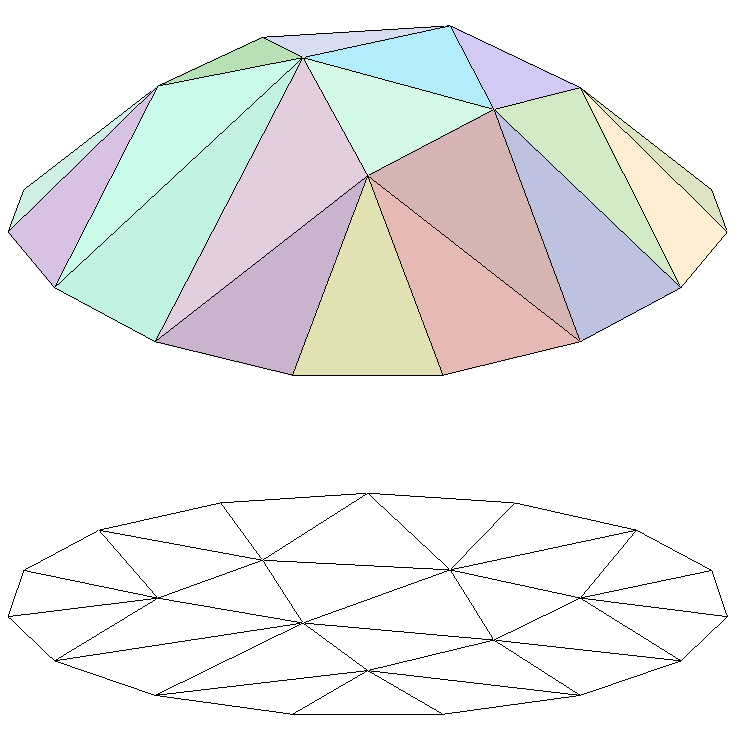
\includegraphics[width=.5\textwidth]{fig/piecewise-linear-function}
    \caption{A piecewise linear finite element function on a
      triangular mesh. Thanks to Oleg Alexandrov on Wikipedia.}
    \label{fig:piecewise-linear}
  \end{figure}
\end{example}

\section{Meshes}

\begin{Definition}{facets}
  Let $\cell\subset \R^d$ be a polyhedron. We call the lower
  dimensional polyhedra constituting its boundary \define{facet}s. A
  facet of dimension zero is called \define{vertex}, of dimension one
  \define{edge}, and a facet of codimension one is called a
  \define{face}.
\end{Definition}

\begin{Definition}{mesh}
  A \define{mesh} $\mesh$ is a nonoverlapping subdivision of the
  domain $\domain$ into polyhedral \define{cell}s denoted by $\cell$,
  for instance simplices, quadrilaterals, or hexahedra. The
  faces of a cell are denoted by $\face$, the
  vertices by $\vertex$. Cells are typically considered open sets.

  A mesh $\mesh$ is called regular, if each face
  $\face \subset \d\cell$ of the cell $\cell\in\mesh$ is either a
  face of another cell $\cell^\prime$, that is,
  $\overline{\face} = \overline{\cell} \cap \overline{\cell^\prime}$,
  or a subset of $\d\domain$.
\end{Definition}

\begin{remark}
  For this introduction, we will assume that indeed $\domain$ is the
  union of mesh cells, which means, that its boundary consists of a
  finite union of planar faces. The more general case of a mesh
  approximating the domain will be deferred to later discussion.
\end{remark}


\section{Local properties of a finite element}

\begin{Definition}{finite-element}
  With a mesh cell $\cell$, we associate a finite dimensional
  \define{shape function} space $\shapespace(\cell)$ of dimension
  $n_\cell$. The term \define{node functional} denotes linear
  functionals used for interpolation to this space.

  A set of node functionals $\{\nodal_\cell^i\}_{i=1,\dots,n_\cell}$ is called
  \define{unisolvent} on $\shapespace(\cell)$ if for any vector
  $\vu = (u_1,\dots,u_{n_\cell})^T$ there exists a unique
  $p\in \shapespace(\cell)$ such that
  \begin{gather}
    \nodal_\cell^i(p) = u_i,\quad i=1,\dots,n_\cell.
  \end{gather}

  A \define{finite element} consists of a mesh cell $T$ with a shape
  function space $\shapespace(\cell)$ and a unisolvent set of node
  functionals.
\end{Definition}

\begin{intro}
  Since we are mostly concerned with finite elements which are
  identical on each cell up to the geometry of the cell, we will drop
  the reference to the cell most of the time and write $\nodal^i$ and
  $\shapespace$.
\end{intro}

\begin{Lemma}{shape-function-basis}
  Let $\nodal^1,\dots,\nodal^{n_{\cell}}$ be the node functionals of the
  finite element and let $\phi_1,\dots,\phi_{n_{\cell}}$ be an arbitrary
  basis of the shape function space.  Let $\matg$ be the Gramian matrix
  between the node functionals and the shape functions with entries
  \begin{gather}
    g_{ik} = \nodal^i(\phi_k).
  \end{gather}
  Then, the set of node functionals is unisolvent on $\shapespace$ if
  and only if $\matg$ is invertible. Furthermore, a
  basis $\{p_k\}$ can be computed by
  \begin{gather}
    \begin{pmatrix}
      p_1(\vx)\\\vdots\\p_{n_{\cell}}(\vx)
    \end{pmatrix}
    = \matg^{-1}
    \begin{pmatrix}
      \phi_1(\vx)\\\vdots\\\phi_{n_{\cell}}(\vx)
    \end{pmatrix},
  \end{gather}
  such that $\nodal^i(p_k) = \delta_{ik}$.
\end{Lemma}

\begin{proof}
  Let for brevity $n=n_{\cell}$. Writing the polynomial $p$ in the
  definition of unisolvence as a linear combination
  \begin{gather}
    p(\vx) = \sum_{k=1}^n a_k \phi_k(\vx),
  \end{gather}
  proving unisolvence reduces to finding a unique coefficient vector
  $\va$ for any vector $\vu$ of node functional evaluations. There holds
  \begin{gather}
    \nodal^i(p)
    = \nodal^i\left(\sum_k a_k\phi_k\right)
    = \sum_k a_k \nodal^i(\phi_k)
    = \sum_k a_k g_{ik}.
  \end{gather}
  Hence, the condition $\nodal^i(p) = u_i$ for $i=1,\dots,n$ amounts
  to the linear system
  \begin{gather}
    \matg\va = \vu,
  \end{gather}
  which has a unique solution for all $\vu$ if and only if $\matg$ is
  invertible. The second statement is confirmed by simple computation.
\end{proof}

\begin{Notation}{dofs}
  If the node functionals $\nodal^i$ are unisolvent on
  $\shapespace(\cell)$, we refer to the basis $\{p_k\}$ of
  $\shapespace(\cell)$ admitting
  \begin{gather}
    \nodal^i(p_k) = \delta_{ik},
  \end{gather}
  as \define{shape function basis}. For any function $u\in C^\infty$,
  it allows to compute the interpolating polynomial
  $p \in \shapespace(\cell)$ by the simple summation
  \begin{gather}
    p(\vx) = \sum_{k=1}^{n_\cell} \nodal^k(u) p_k(\vx).
  \end{gather}
  We use the term \define{degrees of freedom} with a certain
  sloppyness for both the node functionals and the basis functions.
\end{Notation}

\begin{Example}{nodes-linear-triangle}
  The node functionals of the linear triangle in the introduction are the function values in the three vertices.
  \begin{center}
    \includegraphics[width=2cm]{mixed/fig/p1-p.tikz}    
  \end{center}
  The shape function space is the space of linear polynomials $\P_1$
  in two dimensions. The shape function basis consists of the three
  linear polynomials which are one in one of the vertices and zero in
  the other two.
\end{Example}

\section{Global properties of finite elements}

\begin{Definition}{node-topology}
  Node functionals can be associated with the cell $\cell$ or with one
  of its lower dimensional boundary facets. We call these associations
  the \define{topology} of the finite element.

  The global \define{degrees of freedom} are formed by the union of all
  node functionals, where we identify node functionals associated to
  boundary facets among all cells sharing this facet.  
\end{Definition}

\begin{Example*}{nodes-identification}{Identification of node functionals}
  \begin{center}
    \includegraphics[width=.5\textwidth]{graph/concatenation.tikz}    
  \end{center}
  The node functionals on
    shared edges (separated for presentation purposes) are
    distinguished locally as belonging to their respective cells, but
    identical global indices are assigned to all nodes in a single
    circle. Thus, all associated shape functions obtain the same
    coefficient in the global basis representation of a finite element
    function $u$.
\end{Example*}

\begin{intro}
  After the duplicated degrees of freedom on boundary facets of
  adjacent cells have been eliminated, a reduced set of degrees of
  freedom remains. The cardinality of this reduces set determines the
  dimension of the finite element space on the whole mesh.

  For each of those remaining degrees of freedom, we can define a
  basis function for the global finite element space. On each of the
  adjacent cells, it is equal to the shape function associeated with
  the corresponding local degree of freedom.

  After an example, we will formalize this description.
\end{intro}

\begin{Problem}{counting-dofs}
  What are the numbers of degrees of freedom in terms of the
  triangles, edges, and vertices of a mesh for the following local
  node functionals?
  \begin{center}
    \includegraphics[width=2.5cm]{mixed/fig/p1-p.tikz}
    \hspace{10mm}
    \includegraphics[width=2.5cm]{mixed/fig/p2-p.tikz}
    \hspace{10mm}
    \includegraphics[width=2.5cm]{mixed/fig/p3-p.tikz}
  \end{center}
\end{Problem}

\begin{Example*}{shape-basis-functions}{Linear shape and basis functions}
  Given a set of six triangles, we obtain the shape functions
  \begin{center}
    \includegraphics[width=.15\textwidth]{./fig/linear-1.tikz}
    \includegraphics[width=.15\textwidth]{./fig/linear-2.tikz}
    \includegraphics[width=.15\textwidth]{./fig/linear-3.tikz}
    \includegraphics[width=.15\textwidth]{./fig/linear-4.tikz}
    \includegraphics[width=.15\textwidth]{./fig/linear-5.tikz}
    \includegraphics[width=.15\textwidth]{./fig/linear-6.tikz}
  \end{center}
  By identifying the node value at the common vertex, these form a finite element basis function
  \begin{center}
    \includegraphics[width=.4\textwidth]{./fig/linear-hat.tikz}    
  \end{center}
\end{Example*}

\begin{Definition}{fe-space}
  The \define{finite element space} on the mesh $\mesh$, denoted by
  $V_\mesh$ is a subset of the concatenation of all shape function
  spaces,
  \begin{gather}
    V_\mesh \subset \bigl\{ f\in L^2(\domain) \big|
    f_{|\cell} \in \shapespace(\cell) \bigr\}.
  \end{gather}
  
  We choose a basis which has one basis function for each (global)
  degree of freedom (after the elimination above), such that
  \begin{gather}
    \nodal^i(v_k) = \delta_{ik}.
  \end{gather}

  The restriction of this basis function to a cell is the
  corresponding shape function.  The resulting dimension is
  \begin{gather}
    n = \dim V_\mesh \le \sum n_\cell.
  \end{gather}
\end{Definition}

\begin{Notation}{global-local}
  When we enumerate the degrees of freedom of $V_\mesh$, we obtain a
  global numbering of degrees of freedom $\nodal^i$ with
  $i=1,\dots,n$. For each mesh cell, we have a local numbering
  $\nodal_\cell^j$ with $j=1,\dots,n_{\cell}$. By construction of the finite
  element space, there is a unique global index $i$, such that
  $\nodal_\cell^j(f) = \nodal^i(f)$ for all cells $\cell$ and local
  indices $j$. The converse is not true due to the identification
  process.
\end{Notation}

\begin{Definition}{local-global}
  We refer to the mapping between $\nodal^i$ and $\nodal_\cell^j$ as
  the mapping between global and local indices
  \begin{gather}
    \iota: (\cell, j) \mapsto i.
  \end{gather}
  It induces a
  ``natural'' basis $\{v_i\}$ of $V_\mesh$ by
  \begin{gather}
    v_{i|\cell} = p_{\cell,j},
  \end{gather}
  where $\{p_{\cell,j}\}$ is the shape function basis on $\cell$. For
  each $\nodal^i$, we define $\mesh(\nodal^i)$ as the set of cells
  $\cell$ sharing the node functional $\nodal^i$, and
  \begin{gather}
    \domain\left(\nodal^i\right) = \bigcup_{\cell\in \mesh(\nodal^i)} \cell.
  \end{gather}
\end{Definition}

\begin{Lemma}{fe-support}
  The support of the basis function $v_i\in V_\mesh$ is
  \begin{gather*}
    \operatorname{supp}(v_i) \subset \domain\left(\nodal^i\right).
  \end{gather*}
\end{Lemma}

\begin{proof}
  A basis function $v_i$ evaluates to zero at all global node
  functionals $\nodal^j$ for $j\neq i$. Hence, it is zero on all cells
  not sharing $\nodal^i$.
\end{proof}

\begin{Lemma}{mesh-continuity}
  Let $\mesh$ be a subdivision of $\domain$, and let $u$ be a function
  on $\domain$, such that $u_{|\cell} \in C^1(\overline{\cell})$ for
  each $\cell\in\mesh$. Then,
  \begin{gather}
    u\in H^1(\domain)
    \quad \Longleftrightarrow\quad
    u\in C(\overline\domain).
  \end{gather}
\end{Lemma}

\begin{Lemma}{nodal-continuity}
  We have $V_\mesh\subset C(\overline{\domain})$ if and only if for
  every facet $F$ of dimension $d_F < d$ there holds that
  \begin{enumerate}
  \item the trace spaces of the spaces $\shapespace(\cell)$ on $F$ coincide
    for all cells $\cell$ having $F$ as a facet,
  \item the node functionals associated to the facets are identified
    in the right manner between the cells, and
  \item the node functionals associated to the facet are unisolvent on
    this trace space.
  \end{enumerate}
\end{Lemma}

\begin{todo}
  \begin{enumerate}
  \item Introduce the term ``conforming''
  \item Discuss how to identify geometrically identical node functionals!
  \item Example: $H^2$-conforming spaces
  \end{enumerate}
\end{todo}

\begin{Definition}{Galerkin-equations}{Galerkin equations}
  By restricting the weak formulation to the finite element space $V_{\mesh}$, we obtain the \define{Galerkin equations}
  \begin{gather}
    B(u_{\mesh},v_{\mesh}) = \ell(v_{\mesh}) \qquad\forall\;v_{\mesh}\in V_{\mesh}. 
  \end{gather}
  
  After choosing a basis $\{v_i\}$ for $V_{\mesh}$, the Galerkin equations are
  equivalent to a linear system
  \begin{gather}
    \mata \vu = \vf,
  \end{gather}
  with $\mata\in\R^{n\times n}$ and $\vf\in \R^n$ defined by
  \begin{gather}
    a_{ij} = a(v_j, v_i), \qquad f_i = f(v_i).
  \end{gather}
\end{Definition}

\begin{Lemma}{fe-matrix}
  For a finite element discretization of Poisson's equation with the
  space $V_\mesh$, the Galerkin equations can be computed using the
  following formulas:
  \begin{alignat*}3
    a_{ij} &= \int\limits_\domain \nabla v_j \cdot \nabla v_i \dx
    &&= \int\limits_{\domain(\nodal^i)} \nabla v_j \cdot \nabla v_i \dx
    &&= \sum_{\cell\in\mesh(\nodal^i)}\int\limits_\cell \nabla v_j \cdot \nabla v_i \dx\\
    f_{i} &= \int\limits_\domain f v_i \dx
    &&= \int\limits_{\domain(\nodal^i)} f v_i \dx
    &&= \sum_{\cell\in\mesh(\nodal^i)}\int\limits_\cell f v_i \dx
  \end{alignat*}
\end{Lemma}

\begin{Algorithm*}{matrix-assembling}{Assembling the matrix}
  \begin{enumerate}
  \item Start with a matrix $\mata = 0 \in \R^{n\times n}$
  \item Loop over all cells $\cell\in\mesh$
  \item On each cell $\cell$, compute the entries of the cell matrix
    $\mata_\cell \in \R^{n_\cell\times n_\cell}$ by integrating
    \begin{gather}
      a_{\cell,ij} = \int_\cell \nabla p_{\cell,j}\cdot\nabla p_{\cell,i}\,dx,
    \end{gather}
    where $\{p_{\cell,i}\}$ is the shape function basis.
  \item Assemble the cell matrices into the global matrix by
    \begin{gather}
      a_{\iota(i),\iota(j)} = a_{\iota(i),\iota(j)} + a_{\cell,ij}
      \qquad i,j = 1,\dots,n_\cell.
    \end{gather}
  \end{enumerate}
\end{Algorithm*}

\begin{remark}
  \slideref{Lemma}{fe-matrix} and
  \slideref{Algorithm}{matrix-assembling} suggest that the matrix of
  the Galerkin equations is sparse. Indeed, we will always consider
  finite element meshes, where only few elements share a common
  boundary facet. Hence, we can use data structures and algorithms for
  sparse matrices.
\end{remark}

\begin{remark}
  As known from courses in numerical linear algebra, the linear system
  can be solved using an iterative solver, if the mesh consists of
  many cells and the matrix size is huge. For symmetric problems, the
  conjugate gradient method is the solver of choice. We will discuss
  its convergence properties and preconditioning techniques later in
  this class.

  For smaller meshes, a so-called sparse direct solver can be
  used. These compute an LU or Choleski factorization with limited
  fill-in by reordering matrix entries.
\end{remark}

\begin{Example}{Argyris}
  The following finite element is due to Argyris. Take the shape
  function space $\P_5$ and the following node functionals on a
  triangle:
  \begin{itemize}
  \item In each vertex, the function value, the first derivatives, and the second derivatives.
  \item In the midpoint of each edge: the normal derivative.
  \end{itemize}
\end{Example}

\begin{Problem}{Argyris}
  Show that the node functionals of the Argyris element guarantee
  continuously differentiable transitions between mesh cell. To do so,
  follow these steps:
  \begin{enumerate}
  \item In which polynomial space is the trace of a function from the
    shape function space on an edge? The trace of the derivatives?
  \item Show that the node functionals uniquely determine the trace of
    a function on the edge!
  \item Why can we separate the gradient into tangential and normal
    derivatives?
  \item Why are the tangential derivatives continuous?
  \item Show that the node functionals uniquely determine the normal derivatives.
  \end{enumerate}
\end{Problem}

%%%%%%%%%%%%%%%%%%%%%%%%%%%%%%%%%%%%%%%%%%%%%%%%%%%%%%%%%%%%%%%%%%%%%%
%%%%%%%%%%%%%%%%%%%%%%%%%%%%%%%%%%%%%%%%%%%%%%%%%%%%%%%%%%%%%%%%%%%%%%
\section{Shape function spaces on simplices}
%%%%%%%%%%%%%%%%%%%%%%%%%%%%%%%%%%%%%%%%%%%%%%%%%%%%%%%%%%%%%%%%%%%%%%
%%%%%%%%%%%%%%%%%%%%%%%%%%%%%%%%%%%%%%%%%%%%%%%%%%%%%%%%%%%%%%%%%%%%%%

\begin{Definition}{barycentric-coordinates}
  A simplex $\cell\in \R^d$ with vertices $\vertex_0,\dots,\vertex_d$
  is described by a set of $d+1$ \define{barycentric coordinates}
  $\vlambda = (\lambda_0,\dots,\lambda_d)^T$. These are linear functions such that
  \begin{xalignat}2
    0\le\lambda_i(\vx) &\le 1& i&=0,\dots,d;\quad \vx\in\cell\\
    \lambda_i(\vertex_j) &= \delta_{ij}& i,j&=0,\dots,d\\
    \sum \lambda_i(\vx) &= 1,&\vx&\in\cell
  \end{xalignat}
  and there holds
  \begin{gather}
    \cell = \Bigl\{\vx\in\R^d \Big| \vx = \sum \vertex_k\lambda_k(\vx) \Bigr\}.
  \end{gather}
\end{Definition}

\begin{Lemma}{barycentric-affine}
  There is a matrix $B_{\cell}\in \R^{d+1\times d}$ and a vector
  $b_{\cell}\in\R^{d+1}$, such that
  \begin{gather}
    \vlambda = B_{\cell}\vx + b_{\cell}.
  \end{gather}
\end{Lemma}

\begin{proof}
  We give an exemplary proof in two dimensions. There, we have the relation
  \begin{gather}
    \vx = \lambda_0 \vertex_0 + \lambda_1 \vertex_1 + \lambda_2 \vertex_2.
  \end{gather}
  Substituting $\lambda_0 = 1-\lambda_1 - \lambda_2$, we obtain
  \begin{gather}
    \vx = \vertex_0 + (\vertex_1-\vertex_0)\lambda_1 + (\vertex_2-\vertex_0)\lambda_2.
  \end{gather}
  Hence,
  \begin{gather}
    \begin{pmatrix}
      x_1-x_0 & x_2-x_0\\
      y_1-y_0 & y_2-y_0
    \end{pmatrix}
    \begin{pmatrix}
      \lambda_1\\ \lambda_2
    \end{pmatrix}
    =
    \vx - \vertex_0.
  \end{gather}
  The matrix is invertible if the points span a triangle,
  which proves the affine relationship.
\end{proof}

\begin{Corollary}{barycentric-interpolation}
  The barycentric coordinates $\lambda_0,\dots,\lambda_d$ are the
  linear Lagrange interpolating functions for the points
  $\vertex_0,\dots,\vertex_d$. In particular, $\lambda_k \equiv 0$ on
  the facet not containing $\vertex_k$.
\end{Corollary}

\begin{example}
  \label{example:barycentric-shape-functions}
  We can use barycentric coordinates to define interpolating polynomials on
  simplicial meshes easily, as in
  Table~\ref{tab:barycentric-shapes}.
  \begin{table}[tp]
    \centering
    \begin{tabular}{|c|l|}
      \hline Degrees of freedom
      & Shape functions \\\hline
      \adjustbox{valign=center,margin=3pt}{\includegraphics[width=2cm]{mixed/fig/p1-p.tikz}}
      &
        {\begin{minipage}[b]{6cm}
          \begin{gather*}
            \phi_i = \lambda_i,
            \quad i=0,1,2
          \end{gather*}
        \end{minipage}}
      \\\hline
      \adjustbox{valign=center,margin=3pt}{\includegraphics[width=2cm]{mixed/fig/p2-p.tikz}}
      &
        {\begin{minipage}[b]{6cm}
          \begin{xalignat*}2
            \phi_{ii} &= 2\lambda_i^2 - \lambda_i,
            &i&=0,1,2\\
            \phi_{ij} &= 4\lambda_i\lambda_j
            &j&\neq i
          \end{xalignat*}
        \end{minipage}}
        \\\hline
      \adjustbox{valign=center,margin=3pt}{\includegraphics[width=2cm]{mixed/fig/p3-p.tikz}}
      &
        {\begin{minipage}[b]{6cm}
          \begin{xalignat*}2
          \phi_{iii} &= \tfrac12 \lambda_i(3\lambda_i-1)(3\lambda_i-2)
          &i&=0,1,2\\
          \phi_{ijj} &= \tfrac92\lambda_i\lambda_j(3\lambda_j-1)
          &j&\neq i\\
          \phi_{012} &= 27\lambda_0\lambda_1\lambda_2
        \end{xalignat*}
        \end{minipage}}
        \\\hline
    \end{tabular}
    \caption{Degrees of freedom defined as point values in
      interpolation points and shape functions of triangular elements
      in terms of barycentric coordinates}
    \label{tab:barycentric-shapes}
  \end{table}

  The functions $\lambda_i(\vx)$ are the shape functions of the linear
  $P_1$ element on $T$. They allow us to define basis functions on the
  cell $T$ without use of a reference element.

  Note that $\lambda_i\equiv 0$ on the face opposite to the
  vertex $\vx_i$.
  
  We discuss now, why the quadratic functions in the table are the
  shape function basis. First, we observe that at the midpoint
  $\vx_{ij}$ of the edge between $\vx_i$ and $\vx_j$, we have
  $\lambda_i = \lambda_j = \nicefrac12$. Hence,
  $\phi_{ij}(\vx_{ij}) = 1$. Furthermore, this function is zero on
  both other edges, in particular in all other interpolation points.

  The function $\phi_{ii}$ is one for $\lambda_i = 1$ and zero for
  $\lambda_i=\nicefrac12$. Furthermore, it is zero on the opposing
  edge. Hence, it also fulfills the interpolation condition.
\end{example}

\begin{remark}
  The barycentric coordinates of all boundary facets except vertices
  of a simplex are obtained by setting all other barycentric
  coordinates to zero. Hence, if two simplices share a facet, the
  representation of this facet by barycentric coordinates from both
  simplices coincides.

  Since the shape functions are typically provided using the
  barycentric coordinates in a symmetric way, we also obtain a
  reliable way to obtain matching trace spaces from the different
  simplices.
\end{remark}

\begin{example}
  Take the quadratic shape functions in
  Example~\ref{example:barycentric-shape-functions} and their
  restriction to the edge spanned by vertices $\vx_0$ and
  $\vx_1$. Naming the one-dimensional coordinate on the edge
  $t\in[0,1]$, we obtain the basis functions from the table as
  \begin{gather}
    \phi_{00}(t) = 2t^2-t,\qquad
    \phi_{11}(t) = 2(1-t)^2 - (1-t),
    \qquad
    \phi_{01}(t) = 4t(1-t).
  \end{gather}
  These functions are independent of the location of the vertex
  $\vx_2$, and hence coincide for all simplices sharing the edge
  between $\vx_0$ and $\vx_1$.
\end{example}

\begin{remark}
  Vice-versa, we can use this construction to obtain finite elements
  in higher dimension. First, interpolation points and corresponding
  shape functions are fixed on vertices and edges. The shape function
  which eveluates to one in vertex $\vertex_i$ only depends on the
  barycentric coordinate $\lambda_i$. All shape functions for interior
  degrees of freedom on an edge between vertices $\vertex_i$ and
  $\vertex_j$ contain the factor $\lambda_i\lambda_j$, such that they
  vanish in both vertices. Those for triangles with vertices
  $\vertex_i$, $\vertex_j$, and $\vertex_k$ contain the factor
  $\lambda_i\lambda_j\lambda_k$ and vanish on the boundary on the
  triangle. And so on. These functions are sometimes called
  \putindex{bubble function}s, as they look like a bubble on a flat
  surface.
  % Note that the isolines of $\lambda_i$ on a triangle are parallel to
  % the edge opposite to $\vertex_i$. Hence, if we multiply the same linear factors in the interior 
\end{remark}


%%%%%%%%%%%%%%%%%%%%%%%%%%%%%%%%%%%%%%%%%%%%%%%%%%%%%%%%%%%%%%%%%%%%%%
%%%%%%%%%%%%%%%%%%%%%%%%%%%%%%%%%%%%%%%%%%%%%%%%%%%%%%%%%%%%%%%%%%%%%%
\section{Shape functions on quadrilaterals and hexahedra}
%%%%%%%%%%%%%%%%%%%%%%%%%%%%%%%%%%%%%%%%%%%%%%%%%%%%%%%%%%%%%%%%%%%%%%
%%%%%%%%%%%%%%%%%%%%%%%%%%%%%%%%%%%%%%%%%%%%%%%%%%%%%%%%%%%%%%%%%%%%%%

\begin{Definition}{tensor-product-polynomials}
  The space of \define{tensor product polynomials} of degree $k$ in
  $d$ dimensions, denoted as $\Q_k$ consists of polynomials of degree
  up to $k$ in each variable. Given a basis for one-dimensional
  polynomials $\{p_i\}_{i=0,\dots,k}$, a natural basis for $\Q_k$ is
  the \define{tensor product basis}
  \begin{gather}
    \label{eq:fem-intro:1}
    p_{i_1,\dots,i_d}(\vx)
    = p_{i_1}\otimes \dots\otimes p_{i_d}(\vx)
    = \prod_{k=1}^d p_{i_k}(x_k).
  \end{gather}
\end{Definition}

\begin{remark}
  Note that the basis functions of $\Q_k$ can be denoted as products
  of univariate polynomials, but that general polynomials in this
  space as linear combinations of these basis functions do not have
  this structure.
\end{remark}

\begin{Lemma}{tensor-product-node-functionals}
  Let $\{\nodal_j\}$ be a set of one-dimensional node functionals dual
  to the one-dimensional basis $\{p_i\}$ such that
  \begin{gather}
    \nodal_j(p_i) = \delta_{ij}.
  \end{gather}
  Then, a dual basis for $\{p_{i_1,\dots,i_d}\}$ is obtained by
  defining on the tensor product basis of $\Q_k$
  \begin{gather}
    \label{eq:fem-intro:2}
    \nodal_{j_1,\dots,j_d}(p_{i_1,\dots,i_d})
    = \nodal_{j_1} \otimes \dots\otimes \nodal_{j_d}(p_{i_1}\otimes\dots\otimes p_{i_d})
    = \prod_{k=1}^d \nodal_{j_k}(p_{i_k}).
  \end{gather}
\end{Lemma}

\begin{proof}
  It is a theorem in linear algebra, that a linear functional on a
  vector space is uniquely defined by its values on a basis of the
  space. Thus,~\eqref{eq:fem-intro:2} uniquely defines the node
  functionals $\nodal_{j_1,\dots,j_d}$. The duality property follows
  from the fact that
  \begin{gather*}
    \nodal_{j_1,\dots,j_d}(p_{i_1,\dots,i_d}) = \prod_{k=1}^d \delta_{i_k,j_k},
  \end{gather*}
  which is one if and only if all index pairs match and zero in all
  other cases.
\end{proof}

\begin{example}
  Let a basis $\{p_i\}$ of the univariate space $\P_k$ be defined by
  Lagrange interpolation in $k+1$ points $t_j \in [0,1]$. A basis of
  the $d$-dimensional space $\Q_k$ is then obtained by all possible
  products
  \begin{gather*}
    p_{i_1,\dots,i_d}(\vx) = \prod_{k=1}^d p_{i_k}(x_k).
  \end{gather*}
  The node functionals following the construction above are obtained by
  \begin{gather*}
    \nodal_{j_1,\dots,j_d}(p_{i_1,\dots,i_d}) = \prod_{k=1}^d p_{i_k}(x_{j_k}).
  \end{gather*}
  Finally, we have to convert the term on the right into an
  expression, which can be applied to any polynomial in $\Q_k$. To
  this end, we observe that
  \begin{gather*}
    \prod_{k=1}^d p_{i_k}(x_{j_k}) = p_{i_1,\dots,i_d}(x_{j_1},\dots,x_{j_d}).
  \end{gather*}
  Therefore, we conclude that the tensor product node functionals
  resulting from this construction are
  \begin{gather*}
    \nodal_{j_1,\dots,j_d}(p) = p(x_{j_1},\dots,x_{j_d}).
  \end{gather*}
\end{example}

\begin{Example*}{q2}{The space $\Q_2$}
    \begin{center}
    \includegraphics[width=.3\textwidth]{graph/shape0}
    \includegraphics[width=.3\textwidth]{graph/shape1}
    \includegraphics[width=.3\textwidth]{graph/shape2}

    \includegraphics[width=.3\textwidth]{graph/shape3}
    \includegraphics[width=.3\textwidth]{graph/shape4}
    \includegraphics[width=.3\textwidth]{graph/shape5}

    \includegraphics[width=.3\textwidth]{graph/shape6}
    \includegraphics[width=.3\textwidth]{graph/shape7}
    \includegraphics[width=.3\textwidth]{graph/shape8}
  \end{center}
\end{Example*}


\begin{Lemma}{tensor-product-trace}
  The trace of the $d$-dimensional tensor product polynomial space
  $\Q_k$ on the $\delta$-dimensional facets of the reference cube
  $\refcell = (0,1)^d$ is the $\delta$-dimensional space $\Q_k$.

  % The traces from two cells sharing the same face coincide, if the
  % mapping is continuous. Therefore, continuity can be achieved by
  % unisolvent sets of node functionals on the face.
\end{Lemma}

\begin{proof}
  By keeping $d-\delta$ variables constant in the tensor product basis
  in~\eqref{eq:fem-intro:1}.
\end{proof}

\begin{Example*}{cg-q2}{Continuous basis functions}
  \begin{center}
    \includegraphics[height=.20\textwidth]{graph/cgbasis1-02}
    \includegraphics[height=.20\textwidth]{graph/cgbasis1-03}
    \includegraphics[height=.20\textwidth]{graph/cgbasis1-15}
    \includegraphics[height=.20\textwidth]{graph/cgbasis1-16}

    \includegraphics[height=.20\textwidth]{graph/cgbasis1-07}
    \includegraphics[height=.20\textwidth]{graph/cgbasis1-13}
    \includegraphics[height=.20\textwidth]{graph/cgbasis1-18}
    \includegraphics[height=.20\textwidth]{graph/cgbasis1-22}

    \includegraphics[height=.20\textwidth]{graph/cgbasis1-17}
    \includegraphics[height=.20\textwidth]{graph/cgbasis1-23}
    \includegraphics[height=.20\textwidth]{graph/cgbasis1-20}
    \includegraphics[height=.20\textwidth]{graph/cgbasis1-24}
  \end{center}
\end{Example*}

% \begin{Example*}{dg-q2}{Discontinuous basis functions}
%   \begin{center}
%     \includegraphics[height=.20\textwidth]{graph/dgbasis1-08}
%     \includegraphics[height=.20\textwidth]{graph/dgbasis1-15}
%     \includegraphics[height=.20\textwidth]{graph/dgbasis1-20}
%     \includegraphics[height=.20\textwidth]{graph/dgbasis1-27}

%     \includegraphics[height=.20\textwidth]{graph/dgbasis1-07}
%     \includegraphics[height=.20\textwidth]{graph/dgbasis1-19}
%     \includegraphics[height=.20\textwidth]{graph/dgbasis1-23}
%     \includegraphics[height=.20\textwidth]{graph/dgbasis1-30}

%     \includegraphics[height=.20\textwidth]{graph/dgbasis1-26}
%     \includegraphics[height=.20\textwidth]{graph/dgbasis1-33}
%     \includegraphics[height=.20\textwidth]{graph/dgbasis1-24}
%     \includegraphics[height=.20\textwidth]{graph/dgbasis1-22}
%   \end{center}
% \end{Example*}

\begin{example}
  As a second example, we choose $d=2$ and the univariate space $\P_2$ with node functionals
  \begin{gather}
    \nodal_0(p) = p(0),
    \quad \nodal_1(p) = \int_0^1 p(t) \dt,
    \quad \nodal_2(p) = p(1),
  \end{gather}
  that is, a mixture of Lagrange interpolation and orthogonality on
  the interval $[0,1]$. The matching basis polynomials are
  \begin{gather}
    p_0(t) = 3(1-t)^2 - 2(1-t),
    \quad p_1(t) = 6 t(1-t),
    \quad p_2(t) = 3t^2-2t.
  \end{gather}
  Follwoing the construction of the previous example, we obtain
  \begin{gather}
    \begin{aligned}
    \nodal_{00}(p) &= p(0,0),
    &\nodal_{02}(p) &= p(0,1),\\
    \nodal_{20}(p) &= p(1,0),
    &\nodal_{22}(p) &= p(1,1).
    \end{aligned}
  \end{gather}
  Then,
  \begin{gather}
    \nodal_{01}(p_{01}) = \nodal_{01}(p_0\otimes p_1)
    = p_0(0)\int_0^1 p_1(y)\dy
    = \int_0^1 p(0,y) \dy.
  \end{gather}
  Thus, the node functional $\nodal_{01}$ is the integral over the
  left edge of the reference square. By the same construction,
  $\nodal_{01}$ is the integral over the right edge. $\nodal_{10}$ and
  $\nodal_{12}$ are the integrals over the bottom and top edge,
  respectively. Finally,
  \begin{gather}
    \nodal_{11}(p_{11})
    = \int_0^1 p_1(x)\dx \int_0^1 p_1(y) \dy
    = \int_0^1\int_0^1 p_{11}(x,y) \dx\dy.
  \end{gather}
  Thus, the tensor product of two line integrals becomes the integral
  over the area.
\end{example}

%%%%%%%%%%%%%%%%%%%%%%%%%%%%%%%%%%%%%%%%%%%%%%%%%%%%%%%%%%%%%%%%%%%%%%
%%%%%%%%%%%%%%%%%%%%%%%%%%%%%%%%%%%%%%%%%%%%%%%%%%%%%%%%%%%%%%%%%%%%%%
%\section{The Galerkin equations}% and Céa's lemma}
%%%%%%%%%%%%%%%%%%%%%%%%%%%%%%%%%%%%%%%%%%%%%%%%%%%%%%%%%%%%%%%%%%%%%%
%%%%%%%%%%%%%%%%%%%%%%%%%%%%%%%%%%%%%%%%%%%%%%%%%%%%%%%%%%%%%%%%%%%%%%


% \begin{Definition*}{galerkin-approximation}{Galerkin approximation}
%   Let $u\in V$ be determined by the weak formulation
%   \begin{gather*}
%     a(u,v) = f(v) \qquad\forall v\in V,
%   \end{gather*}
%   where $V$ is a suitable function space including boundary
%   conditions. The \define{Galerkin approximation}, also called
%   \define{conforming approximation} of this problem reads as follows:
%   choose a subspace $V_n\subset V$ of dimension $n$ and find
%   $u_n\in V_n$, such that
%   \begin{gather*}
%     a(u_n,v_n) = f(v_n) \qquad\forall v_n\in V_n.
%   \end{gather*}
%   We will refer to this equation as the \define{discrete problem}.
% \end{Definition*}


% \begin{Lemma}{discrete-lax-milgram}
%   If the lemma of Lax-Milgram holds for $a(.,.)$ on $V$, it holds on
%   $V_n\subset V$. In particular, solvability of the Galerkin equations
%   is implied.
% \end{Lemma}

% \begin{proof}
%   Since coercivity and boundedness hold for all $u,v\in V$ they hold
%   in particular for all $u,v\in V_n$.
% \end{proof}

% \begin{Lemma}{galerkin-ortho}
%   Let $a(.,.)$ be a bilinear form on the Hilbert
%   space $V$.
%   Let $u \in V$ and $u_n\in V_n \subset V$ be the solution to the
%   weak formulation and its Galerkin approximation
%   \begin{gather*}
%     \begin{aligned}
%       a(u,v) &= f(v) & \qquad\forall v&\in V,\\
%       a(u_n,v_n) &= f(v_n) & \qquad\forall v_n&\in V_n,
%     \end{aligned}
%   \end{gather*}
%   respectively. Then, there holds the \define{Galerkin orthogonality}
%   \begin{align}
%     \label{eq:galerkin-ortho}
%     a(u-u_n,v_n) = 0 \qquad \forall v_n\in V_n.
%   \end{align}
% \end{Lemma}

% \begin{proof}
%   As $v_n\in V_n$ there holds $a(u,v_n)=f(v_n)$, too.
%   Then, there holds for an arbitrary $v_n\in V_n$
%   \begin{gather*}
%     a(u-u_n,v_n)=a(u,v_n)-a(u_n,v_n)=f(v_n)-f(v_n)=0.
%   \end{gather*}
% \end{proof}

% \begin{Lemma*}{cea}{Céa}
%   Let $a(.,.)$ be a bounded and elliptic bilinear form on the Hilbert
%   space $V$.  Let $u \in V$ and $u_n\in V_n \subset V$ be
%   the solution to the weak formulation and its Galerkin approximation
%   respectively. Then, there holds
%   \begin{gather}
%     \norm{u-u_n}_V \le \frac{M}{\alpha}
%     \inf_{v_n\in V_n}\norm{u-v_n}_V.
%   \end{gather}
% \end{Lemma*}

% \begin{proof}
%   As $a(.,.)$ is coercive with $\alpha>0$ and bounded with $M>0$
%   we get for arbitrary $v_n\in V_n$
%   \begin{gather*}
%     \begin{aligned}
%       \alpha \norm{u-u_n}_V^2 &\le a(u-u_n,u-u_n) = a(u-u_n,u-v_n+v_n-u_n) \\
%       &= a(u-u_n,u-v_n) + \underbrace{a(u-u_n,v_n-u_n)}_{=0} \\
%       &\le M \norm{u-u_n}_V \norm{u-v_n}_V.
%     \end{aligned}
%   \end{gather*}
%   In the second line we applied the Galerkin orthogonality
%   as $v_n-u_n\in V_n$. Dividing by $\norm{u-u_n}_V$ there holds
%   \begin{gather*}
%     \norm{u-u_n}_V \leq \frac{M}{\alpha} \norm{u-v_n}_V.
%   \end{gather*}
%   As $v_n\in V_n$ was chosen arbitrary, we conclude
%   \begin{gather*}
%     \norm{u-u_n}_V \le \inf_{v_n\in V_n} \norm{u-v_n}_V.
%   \end{gather*}
% \end{proof}

\begin{remark}
  There remains the problem from the homework. Depending on the
  orientation of a quadrilateral, the node functionals provided by
  interpolation in the four corners are not unisolvent. Hence, we will
  reconsider our introduction of shape function spaces in the next
  section.
\end{remark}

%%%%%%%%%%%%%%%%%%%%%%%%%%%%%%%%%%%%%%%%%%%%%%%%%%%%%%%%%%%%%%%%%%%%%%
%%%%%%%%%%%%%%%%%%%%%%%%%%%%%%%%%%%%%%%%%%%%%%%%%%%%%%%%%%%%%%%%%%%%%%
\section{Mapped finite elements}
%%%%%%%%%%%%%%%%%%%%%%%%%%%%%%%%%%%%%%%%%%%%%%%%%%%%%%%%%%%%%%%%%%%%%%
%%%%%%%%%%%%%%%%%%%%%%%%%%%%%%%%%%%%%%%%%%%%%%%%%%%%%%%%%%%%%%%%%%%%%%

\begin{Definition}{mapped-mesh}
  A mapped mesh $\mesh$ is a set of cells $\cell$, which are defined
  by a single \define{reference cell} $\refcell$ and individual
  smooth mappings
  \begin{gather}
    \begin{split}
      \Phi_\cell \colon \refcell &\to \R^d\\
      \Phi_\cell(\refcell) &= \cell.
    \end{split}
  \end{gather}
  The definition extends to small sets of reference cells, for
  instance for triangles and quadrilaterals.
\end{Definition}

\begin{Example}{mapping-linear}
  Let the reference triangle $\refcell$ be defined by
  \begin{gather}
    \refcell = \left\{
      \begin{pmatrix}
        \refx\\\refy
      \end{pmatrix}
      \middle|
      \refx,\refy >0, \refx+\refy < 1
    \right\}.
  \end{gather}
  Then, every cell $\cell$ spanned by the vertices $\vertex_0$,
  $\vertex_1$, and $\vertex_2$ is obtained by mapping $\refcell$ by
  the \putindex{affine mapping}
  \begin{gather}
    \Phi_\cell(\refvx) =
    \begin{pmatrix}
      X_1-X_0 & X_2 - X_0 \\ Y_1-Y_0 & Y_2 - Y_0
    \end{pmatrix}
    \begin{pmatrix}
      \refx \\ \refy
    \end{pmatrix}
    +
    \begin{pmatrix}
      X_0 \\ Y_0
    \end{pmatrix} =: \matb_\cell \refvx + \vb_\cell
  \end{gather}
  This definition extends to simplices in any dimension.
\end{Example}

\begin{Example}{mapping-bilinear}
  The reference cell for a quadrilateral is the reference square
  $\refcell = (0,1)^2$. Every quadrilateral $\cell$ spanned by the
  vertices $\vertex_0$ to $\vertex_3$ is then obtained by the
  \putindex{bilinear mapping}
  \begin{gather}
    \Phi_\cell(\refvx)
    = \bigl[\vertex_0 (1-\refx)
    + \vertex_1 \refx\bigr] (1-\refy)
    + \bigl[\vertex_2 (1-\refx)
    + \vertex_3 \refx\bigr]\refy.
  \end{gather}
\end{Example}

\begin{Example}{mapping-trilinear}
  In three dimensions, the reference for a hexahedral mesh is the
  reference cube $\refcell = (0,1)^3$. The \putindex{trilinear
    mapping} to the mesh cell $\cell$ spanned by the vertices
  $\vertex_0$ to $\vertex_7$ is a straightforward extension of the
  bilinear mapping, namely
  \begin{gather}
    \begin{split}
      \Phi_\cell(\refvx)
      &= \Bigl[\bigl[\vertex_0 (1-\refx)
      + \vertex_1 \refx\bigr] (1-\refy)
      + \bigl[\vertex_2 (1-\refx)
      + \vertex_3 \refx\bigr]\refy\Bigr] (1-\refz)\\
      &+ \Bigl[\bigl[\vertex_4 (1-\refx)
      + \vertex_5 \refx\bigr] (1-\refy)
      + \bigl[\vertex_6 (1-\refx)
      + \vertex_7 \refx\bigr]\refy\Bigr] \refz.      
    \end{split}
  \end{gather}
  Note that in this case the faces of the cell $\cell$ are in general
  not planar, but bilinear surfaces.
\end{Example}

\begin{Definition}{mapped-fe}
  Mapped shape functions $\{p_i\}$ on a mesh cell $\cell$ are defined by a
  set of shape functions $\{\refp_i\}$ on the reference cell
  $\refcell$ through \define{pull-back}
  \begin{gather}
    \begin{split}
      p_i(\vx) &= \refp_i\left(\Phi^{-1}(\vx)\right) = \refp_i(\refvx),\\
      \nabla p_i(\vx) &= \nabla\Phi^{-T}(\refvx)\refgrad\refp_i(\refvx)
    \end{split}
  \end{gather}
\end{Definition}

\begin{remark}
  Using mapped finite elements also opens a new avenue for computing
  the integrals needed to form the Galerkin equations. Since we can
  now integrate over the reference cell $\refcell$, we can use
  tabulated quadrature formulas instead of computing integrals by
  hand.
\end{remark}


\begin{Lemma}{mapped-norms-affine}
  Let $\refcell$ be the reference triangle and let $\cell$ be a
  triangular mesh cell with mapping
  $\vx = \Phi_\cell(\refvx) = \matb \refvx + \vb$. Let there hold
  $u(\vx) = \refu(\refvx)$. Then, $u\in H^k(\cell)$ if and only if
  $\refu\in H^k(\refcell)$ and we have with some constant $c$ the
  estimates
  \begin{gather}
    \begin{split}
      \snorm{\refu}_{k,\refcell}
      &\le c \norm{\matb}^k (\det \matb)^{-\nicefrac12}
      \snorm{u}_{k,\cell},\\
      \snorm{u}_{k,\cell}
      &\le c \norm{\matb^{-1}}^k (\det \matb)^{\nicefrac12}
      \snorm{\refu}_{k,\refcell}.
    \end{split}
  \end{gather}
\end{Lemma}

\begin{Lemma}{shape-regular-transformation}
  For a cell $\cell$, let $R$ be the radius of the circumscribed
  circle and $\rho$ the radius of the inscribed circle. Then,
  \begin{gather}
    \norm{\matb} \le c R, \qquad \norm{\matb^{-1}} \le c \rho^{-1}.
  \end{gather}
\end{Lemma}

\begin{proof}
  \begin{figure}
    \centering
    \begin{tikzpicture}
    \def\scale{3}
    
    %% reference cell
    \def\mid{\scale*0.2928932188}
    \def\outermid{\scale*0.5}
    \def\outerrad{\scale*0.7071067811}
    
    \node (mid) at (\mid,\mid) {$\refvx_0$};
    \coordinate (x1) at (\scale*1,0);
    \node[right = \scale*0.01 of x1] (x1name) {$\refvx_1$};
    \coordinate (x2) at (0,\scale*1);
    \node[above = \scale*0.01 of x2] (x2name) {$\refvx_2$};
    \coordinate (x3) at (0,0);
    \node[left = \scale*0.01 of x3] (x3name) {$\refvx_3$};
    \coordinate (xc) at (\outermid,\outermid);
    \node[above = \scale*0.01 of xc] (xcname) {$\refvx_c$};
    
    \draw (x1)--(x2)--(x3)--(x1);
    
    % incircle
    \draw (mid) circle (\mid);
    \draw (mid) --  (\mid,0);
    \node[below = \scale*0.01 of mid,xshift=0.5em] (rho) {$\refrho$};
    
    % circumcircle
    \draw (xc) circle (\outerrad);
    \draw (xc) -- (\outermid+\outerrad,\outermid);
    \node[above right = \scale*0.01 and \scale*0.25 of xc] (R) {$\reference{R}$};
    \end{tikzpicture}
    \caption{Visualization of the inscribed and circumscribed circle of the reference cell $\refcell$.}
  \end{figure}

  Let us define $S_{\refrho}\coloneqq \{\refvy\in\R^d ~\mid~ \abs{\refvy}=\refrho \}$.
  For $\refvy\in S_{\refrho}$ there holds
  $\refvx\coloneqq \refvxo + \refvy\in \overline{\refcell}$
  and $\vx=\matb\refvx + \vb = \matb(\refvxo+\refvy)+\vb$.
  Additionally, we have $\vxo = \matb \refvxo + \vb$
  which yields
  \begin{align*}
    \abs{\vx-\vxo} = \abs{\matb\refvy}\leq 2R.
  \end{align*}
  Now consider the operator norm of $\matb$
  \begin{align*}
    \norm{\matb} = \sup_{\refvy\in\R^d} \frac{\abs{\matb\refvy}}{\abs{\refvy}}
    = \sup_{\abs{\refvy}=1} \abs{\matb\refvy}
    = \sup_{\refvy\in S_{\refrho}} \frac{\abs{\matb\refvy}}{\refrho}
    \leq \frac{2R}{\refrho}.
  \end{align*}
  $\refrho$ is a constant only depending on $\refcell$ but
  not on $\cell$. Hence, we get $\norm{\matb}\leq cR$ with $c$ depending
  on $\refrho$.

  The same argument can be applied for the second estimate.
  We now define $S_\rho\coloneqq \{\vy\in\R^d~\mid~\abs{\vy}=\rho \}$.
  For $\vy\in S_\rho$ there holds $\vx\coloneqq\vxo+\vy\in\overline{\cell}$
  and let $\refvx=\matb^{-1}\vx-\vb,~\refvxo=\matb^{-1} \vxo - \vb$ which yields
  \begin{align*}
    \abs{\refvx - \refvxo} = \abs{\matb^{-1} \vy}\leq 2\reference{R}.
  \end{align*}
  Analogous to the first estimate we obtain
  \begin{align*}
    \norm{\matb^{-1}} = \sup_{\vy\in S_\rho} \frac{\abs{\matb^{-1} \vy}}{\rho}
    \leq \frac{2\reference{R}}{\rho}.
  \end{align*}
  Now $\reference{R}$ is only depending on $\refcell$ but not on $\cell$.
  Hence, we have $\norm{\matb^{-1}}\leq c\rho^{-1}$ where $c$ depends
  on $\reference{R}$.
\end{proof}

\begin{Assumption}{mapping-decomposition}
  For more general mappings $\Phi\colon \refcell\to \cell$, we
  make the assumption, that they can be decomposed into three factors,
  \begin{gather}
    \Phi = \Phi_O \circ \Phi_S \circ \Phi_W,
  \end{gather}
  where $\Phi_O$ is a combination of translation and rotation,
  $\Phi_S$ is a scaling with a characteristic length $h_{\cell}$, and
  $\Phi_W$ is a warping function not changing the characteristic length.
\end{Assumption}

\begin{example}
  We construct the inverse of $\Phi$ in two dimensions by the
  following three steps, using as $h_\cell$ the length of the longest
  edge of $\cell$.
  \begin{enumerate}
  \item Choose $\Phi_O$ as the rigid body movement which maps the
    longest edge to the interval $(0,h_\cell)$ on the $x$-axis and the
    cell itself to $\cell_O$ in the positive half plane. This mapping
    has the structure
    \begin{gather*}
      \Phi^{-1}_O (\vx) = \mats \vx - \mats \vertex_0,
    \end{gather*}
    where $\mats$ is an orthogonal matrix and $\vertex_0$ is the
    vertex moved to the origin.
  \item Choose the scaling
    \begin{gather*}
      \Phi^{-1}_S (\vx) = \tfrac1{h_\cell} \vx,
    \end{gather*}
    such that the longest edge of the resulting cell $\cell_S$ has the
    longest edge equal to the interval $(0,1)$ on the $x$-axis.
  \item Warp the cell $\cell_S$ into the reference cell $\refcell$ by
    the mapping $\Phi^{-1}_W$. This operation leaves the longest edge
    untouched. For triangles, it is the uniquely defined linear
    transformation mapping the vertex not on the longest edge to
    $(0,1)$. For quadrilaterals, it is a bilinear transformation.
  \end{enumerate}

  In the first step, we have assumed that the cell is convex, which is
  always true for triangles. For nonconvex quadrilaterals, it can be
  shown that the determinant of $\nabla\Phi$ changes sign inside the
  cell, such that these cells are not useful for computations.

  The idea of this decomposition is, that we separate mappings
  changing the position, size, and shape of the cells.
\end{example}

\begin{Lemma*}{scaling-1}{Scaling lemma}
  Let the typical length of a cell $\cell$ be $h_\cell$. Assume there
  are constants $0 < M_\cell, m_\cell, d_\cell, D_\cell$, such that
  \begin{gather}
    \begin{split}
      \norm{\nabla\Phi_W(\refvx)} \le M_\cell,
      \\
      \norm{\nabla\Phi_W^{-1}(\refvx)} \le m_\cell^{-1} ,
      \\
      d^2_\cell \le \det \nabla\Phi_W(\refx)) \le D^2_\cell.      
    \end{split}
  \end{gather}
  for all $\refvx\in\refcell$. Then, for $k=0,1$ and a constant $c$
  \begin{gather}
    \begin{split}
      \snorm{\refu}_{k,\refcell}
      &\le c \frac{M_\cell}{d_\cell}  h_\cell^{k-\nicefrac d2}
      \snorm{u}_{k,\cell},\\
      \snorm{u}_{k,\cell}
      &\le c \frac{D_\cell}{m_\cell} h_\cell^{\nicefrac d2-k}
      \snorm{\refu}_{k,\refcell}.
    \end{split}
  \end{gather}
  This extends to higher derivatives under assumptions on higher
  derivatives of $\Phi_\cell$.
\end{Lemma*}

\begin{proof}
  By the chain rule,
  $\nabla \Phi_{\cell} = \nabla \Phi_O \nabla \Phi_S \nabla \Phi_W$. By
  construction, $\nabla\Phi_O$ is an orthogonal matrix, such that
  \begin{gather*}
    \norm{\nabla\Phi_O} = \norm{\nabla\Phi_O^{-1}} = 1.
  \end{gather*}
  Since it preserves angles and lengths, $\det \nabla\Phi_O =
  1$. Since $\Phi_S$ is a multiple of the identity, we have
  \begin{gather*}
    \norm{\nabla\Phi_S} = h_\cell,
    \quad\norm{\nabla\Phi_S^{-1}} = \frac1{h_\cell},
    \quad\det\nabla\Phi_S = h_\cell^d.
  \end{gather*}
  By change of variables, we have
  \begin{gather*}
    \int_\cell u^2 \dvx
    = \int_{\refcell} \refu^2 \abs{\det\nabla\Phi_\cell} \dvxref
    = \int_{\refcell} \refu^2 \det\nabla\Phi_S\det\nabla\Phi_O\det\nabla\Phi_W \dvxref
    ,
  \end{gather*}
  such that the case $k=0$ is proven immediately by
  \begin{gather*}
    h_{\cell}^d d_\cell^2 \int_{\refcell} \refu^2 \dvxref
    \le \int_\cell u^2 \dvx
    \le h_{\cell}^d D_\cell^2 \int_{\refcell} \refu^2 \dvxref
  \end{gather*}
  By the chain rule, we have
  \begin{gather*}
    \refgrad\refu(\refvx) = \nabla\Phi^T \nabla u(\vx)
    = \nabla\Phi_W^T \nabla\Phi_S^T \nabla\Phi_O^T \nabla u(\vx),
  \end{gather*}
  such that there holds
  \begin{gather}
    \begin{split}
      \abs{\refgrad\refu(\refvx)}
      &\le \norm{\nabla\Phi_W} h_\cell \abs{\nabla u},\\
      \abs{\nabla u(\vx)}
      &\le \norm{\nabla\Phi_W^{-1}} h_\cell^{-1} \abs{\refgrad \refu}.
    \end{split}
  \end{gather}
\end{proof}


\begin{Remark}{simple-mappings}
  We have $d_\cell = D_\cell$, if and only if the mapping is
  affine. The quotient $M_\cell/m_\cell$ measures how much the shape
  of the mesh cell deviates from the reference cell. For instance, it
  is one for squares.
\end{Remark}

%%%%%%%%%%%%%%%%%%%%%%%%%%%%%%%%%%%%%%%%%%%%%%%%%%%%%%%%%%%%%%%%%%%%%%
%%%%%%%%%%%%%%%%%%%%%%%%%%%%%%%%%%%%%%%%%%%%%%%%%%%%%%%%%%%%%%%%%%%%%%
\section{Essential boundary conditions}
%%%%%%%%%%%%%%%%%%%%%%%%%%%%%%%%%%%%%%%%%%%%%%%%%%%%%%%%%%%%%%%%%%%%%%
%%%%%%%%%%%%%%%%%%%%%%%%%%%%%%%%%%%%%%%%%%%%%%%%%%%%%%%%%%%%%%%%%%%%%%

\begin{intro}
  In the introduction of weak formulations, we have seen that
  Dirichlet boundary conditions are modeled by modifying the function
  space, for instance by replacing $H^1(\domain)$ by
  $H^1_0(\domain)$. In this section, we discuss the application of
  this concept in the context of finite element spaces.
\end{intro}

%%% Local Variables: 
%%% mode: latex
%%% TeX-master: "main"
%%% End: 

\section{A priori error analysis}
\input{fem-apriori}
\section{A posteriori error analysis}
\input{fem-aposteriori}

\chapter{Variational Crimes}
\begin{intro}
  In the previous chapter, we considered finite element methods
  applying the original bilinear form to a subspace $V_h\subset
  V$. This assumes, that the domain $\domain$ is exactly represented
  by the mesh, and that all integrals are computed exactly. Both
  assumptions reduce the applicability of the finite element method
  considerably. Therefore, we now extend our analysis to cases, where
  we allow $V_h \not\subset V$ and discrete bilinear forms
  $a_h(.,.) \neq a(.,.)$.
\end{intro}

\section{Numerical quadrature}
\input{quadrature}

\chapter{Solving the Discrete Problem}
\input{iteration/itintro}
\input{iteration/richardson}
\input{iteration/cg}

\section{Condition numbers of finite element matrices}
\begin{Notation}{up-to-a-constant}
  In asymptotic estimates, we will use the notation
  \begin{gather*}
    a \lesssim b \qquad\text{and}\qquad b \gtrsim a,
  \end{gather*}
  if there is a constant c independent of the relevant quantities, such that
  \begin{gather*}
    a \le c \,b\qquad\text{and}\qquad c\,b \ge a.
  \end{gather*}
  We use
  \begin{gather*}
    a \simeq b,
  \end{gather*}
  if both hold. The latter is more precise than $a = \mathcal O(b)$,
  since it implies the same asymptotic order.
\end{Notation}

% \begin{example}
%   The interpolation estimate~\eqref{eq:fe-interpolation} could be written as
%   \begin{align*}
%     \norm{u-I_h u}_{m;h} \lesssim h^{k+1-m} \snorm{u}_{k+1;h},\\
%     \intertext{instead of}
%     \norm{u-I_h u}_{m;h} \le c h^{k+1-m} \snorm{u}_{k+1;h}.
%   \end{align*}
%   The statement of the equivalence of two norms becomes
%   \begin{gather*}
%     \norm{\cdot}_X \simeq \norm{\cdot}_Y,
%   \end{gather*}
%   while 
%   \begin{gather*}
%     \norm{\cdot}_X \lesssim \norm{\cdot}_Y
%   \end{gather*}
%   states that the $Y$-norm is not weaker than the $X$-norm.
% \end{example}

\begin{Definition}{mass-stiffness}
  Let $\mesh_h$ be a mesh on the domain $\domain$ and $V_h$ a finite
  element space with basis $\{\phi_i\}$. Then, the matrix associated
  with the $L^2$-inner product with entries
  \begin{gather*}
    m_{ij} = \int_\Omega \phi_j(x) \phi_i(x) \dx,
  \end{gather*}
  is called \define{mass matrix}.
  The matrix associated with the
  bilinear form of the equation is called \define{stiffness matrix},
  \begin{gather*}
    a_{ij} = a(\phi_j,\phi_i).
  \end{gather*}
\end{Definition}

\begin{Lemma}{condition-number-mass-matrix}
  Let $\{\phi_i\}$ be the basis of a finite element shape function
  space on a quasi-uniform family of meshes $\{\mesh_h\}$. Let
  $\matm_h$ be the mass matrix. Then,
  \begin{gather*}
    \Lambda(\matm) \simeq h^{d} \simeq  \lambda(\matm)
  \end{gather*}
  Therefore, the condition number is (asymptotically in $h$)
  \begin{gather*}
    \kappa(\matm) \simeq 1.
  \end{gather*}
\end{Lemma}

\begin{proof}
  % It is easy to verify, that $m_{ii}> 0$, and that there are not more
  % entries in each row as edges of the triangulation meet in one vertex
  % are different from zero. Furthermore, that the size of those entries
  % is of order $h^d$, where $d$ is the space dimension. From these two
  % facts we immediately obtain
  % \begin{gather*}
  %   \Lambda(\matm) = \mathcal O(h^{d}).
  % \end{gather*}
  % The argument for $\lambda(\matm)$ is more subtle. 
  For any mesh cell
  $\cell\in\mesh_h$, let $\vecx_{\cell}$ be the entries of the vector $\vecx$ which
  belong to node values of the cell $\cell$. Let $\matm_\cell$ be the cell
  mass matrix obtained by restricting the $L^2$-inner product to
  $\cell$. Then,
  \begin{gather*}
    % \norm{u_h}_{L^2(\domain)}^2
    \vecx^T \matm_h \vecx
    = \sum_{\cell\in\T_h} \vecx^T_{\cell} \matm_{\cell} \vecx_{\cell}
    \begin{cases}
    \ge \min\limits_{\cell\in\T_h} \frac{\vecx^T_{\cell} \matm_{\cell} \vecx_{\cell}}{\abs{\vecx_{\cell}}} \sum_{\cell\in\T_h} \abs{\vecx_{\cell}}^2 \ge \lambda(\matm_{\cell}) \abs{\vecx}^2,\\
    \le \max\limits_{\cell\in\T_h} \frac{\vecx^T_{\cell} \matm_{\cell} \vecx_{\cell}}{\abs{\vecx_{\cell}}} \sum_{\cell\in\T_h} \abs{\vecx_{\cell}}^2 \le c \Lambda(\matm_{\cell}) \abs{\vecx}^2,
    \end{cases}
  \end{gather*}
  where the constant in the upper bound is due to degrees of freedom
  shared by different elements. Dividing by $\abs{\vecx}^2$, we
  obtain
  \begin{gather}
    \lambda(\matm_\cell) \le \frac{\vecx^T \matm_h \vecx}{\abs{\vecx}^2} \le c \Lambda(\matm_\cell).
  \end{gather}
  In order to estimate the eigenvalues of $\matm_{\cell}$, we note that for
  a unisolvent element, the norms $\abs{\vecx_{\cell}}$ and $\norm{u}_{0,T}$ are
  equivalent on the reference cell, and the $L^2$-norm scales with
  $h^d$ when transforming to the real cell $T$. Thus, we have
  $\lambda(\matm_h) = \mathcal O(h^{d}) = \Lambda(\matm_h)$.
\end{proof}

\begin{Corollary}{refined-condition-number}
  Let $\mesh_h$ be a shape-regular mesh with cell sizes ranging
  between the minimum $h$ and the maximum $H$. Then, we have
  \begin{align*}
    \Lambda(\matm) &\simeq H^{d} \\
    \lambda(\matm) &\simeq h^{d} \\
    \kappa(\matm) &\simeq \left(\frac Hh\right)^{d}
  \end{align*}
\end{Corollary}

\begin{remark}
  We have only computed the dependence of the condition number on the
  mesh size $h$, not on the polynomial degree of the shape function
  space. Indeed, the used equivalence between the $L^2$-norm of a
  polynomial on the reference cell and the Euclidean norm of its
  coefficient vector depends not only on the degree of the shape
  function space, but on its basis.
\end{remark}

\begin{Theorem}{condition-number-stiffness-matrix}
  Let $\{\phi_i\}$ be the nodal basis of a finite element shape
  function space on a quasi-uniform family of meshes
  $\{\mesh_h\}$. Let $\mata_h$ be the stiffness matrix of the
  Laplacian with Dirichlet boundary values.  Then,
  \begin{gather*}
    \Lambda(\mata) \simeq h^{d-2}, \qquad \lambda(\mata)  \simeq h^{d}
  \end{gather*}
  Therefore, the condition number is
  \begin{gather*}
    \kappa(\matm) \simeq h^{-2}.
  \end{gather*}
\end{Theorem}

\begin{proof}
  First, we investigate the largest eigenvalue. By the scaling
  argument, there holds $a_{ij} \simeq h^{d-2}$. Since by the
  Gershgorin theorem all eigenvalues are bounded by the sum of the
  elements in a row, and this number is bounded uniformly on shape
  regular meshes, we have $\Lambda(\mata_h) \lesssim h^{d-2}$. Now, we
  choose a particular example, namely a vector $\vecx$ with a single one and
  all other entries zero. The corresponding finite element function
  $u_h$ has maximum one and support of radius $h$. Therefore,
  \begin{gather*}
    \vecx^T\mata_h\vecx=
    \int_\domain \abs{\nabla u_h}^2 \dvx
    \simeq h^{d-2}.
  \end{gather*}
  Thus, $\Lambda(\mata_h) \gtrsim h^{d-2}$. In order to estimate the
  smallest eigenvalue, we use the Rayleigh quotient and the finite
  element function $u_h$ corresponding to the coefficient vector
  $\vecx$ to obtain
  \begin{multline}
    \lambda(\mata_h)
    = \min_{\vecx\in\R^n}\frac{\vecx^T\mata_h\vecx}{\vecx^T\vecx}
    = \min_{\vecx\in\R^n}\frac{\vecx^T\mata_h\vecx}{\form(u_h,u_h)_{L^2}}
    \frac{\form(u_h,u_h)_L^2}{\vecx^T\vecx}
    \\
    = \min_{\vecx\in\R^n}\left(\frac{a(u_h,u_h)}{\form(u_h,u_h)}
    \frac{\vecx^T\matm_h\vecx}{\vecx^T\vecx}\right)
    \ge \min_{u_h\in V_h}\frac{a(u_h,u_h)}{\form(u_h,u_h)_L^2}
    \min_{\vecx\in\R^n}\frac{\vecx^T\matm_h\vecx}{\vecx^T\vecx}.
  \end{multline}
  Thus, the smallest eigenvalue of $\mata_h$ is bounded by the product
  of the smallest eigenvalue of the mass matrix and a value $\mu$ given by
  \begin{gather}
    \min_{u_h\in V_h}\frac{a(u_h,u_h)}{\form(u_h,u_h)_L^2} \ge
    \min_{u\in V}\frac{a(u,u)}{\form(u,u)_L^2} =: \mu.
  \end{gather}
  Here, we need a result from the spectral analysis of the
  Laplacian. When we define the variational eigenvalue problem
  \begin{gather}
    a(u,v) = \lambda \form(u,v)\qquad\forall v\in V = H^1_0(\domain),
  \end{gather}
  then, there is a positive minimal solution $\mu$, the first
  eigenvalue of the Laplacian, and an associated eigenfunction $u$,
  such that the equation holds for all $v$. Therefore, the eigenvalue
  is bounded with $\lambda(\mata_h) \gtrsim h^{-d}$. Furthermore, it
  can be shown that this function is smooth and does not
  oscillate. This actually follows from the regularity result in
  \slideref{Theorem}{gt-8-13}. Therefore, the solution $u_h\in V_h$ to
  \begin{gather}
    a(u_h, v_h) = a(u,v_h) \qquad\forall v_h\in V_h,
  \end{gather}
  converges to $u$ in $H^1$ and $L^2$. With our standard estimates, we obtain
  \begin{gather}
    \form(u, u_h)
    = \form(u_h,u_h) + \form(u-u_h,u_h)
    = \form(u_h,u_h) + r_h(u),
  \end{gather}
  where $r_h(u)\to 0$ as $h\to 0$. Hence,
  \begin{gather}
    a(u_h,u_h) = a(u,u_h) = \mu \form(u,u_h) \to \mu \form(u_h,u_h).
  \end{gather}
  We conclude that the lower bound for the eigenvalue is sharp and the
  theorem holds.
\end{proof}

%%% Local Variables:
%%% mode: latex
%%% TeX-master: "main"
%%% End:


\section{Multigrid methods}
\def\restrict{r}
\def\prolongate{p}
\begin{example}
  Smoothing property of the Gauss-Seidel method for the one-dimensional Laplacian.
  \begin{figure}[tp]
    \begin{center}
      \includegraphics[width=.49\textwidth]{../graph/smoothing/gauss-seidel-0.tikz}
      \includegraphics[width=.49\textwidth]{../graph/smoothing/gauss-seidel-3.tikz}
      \includegraphics[width=.49\textwidth]{../graph/smoothing/gauss-seidel-1.tikz}
      \includegraphics[width=.49\textwidth]{../graph/smoothing/gauss-seidel-4.tikz}
      \includegraphics[width=.49\textwidth]{../graph/smoothing/gauss-seidel-2.tikz}
      \hbox to .49\textwidth{}
    \end{center}
    \caption{Development of the error of the Gauss-Seidel iteration. Random initial error and errors after one and two steps (left). Errors after 3, 4, and 5 steps (top right) and after 10, 20, 40, 80, 160, and 320 steps (lower right).}
  \end{figure}
\end{example}
\begin{Algorithm*}{mgm}{The Multigrid iteration MGM($\ell, u_\ell^{k}, b_\ell$)}
  \index{multigrid iteration}
  \begin{enumerate}
  \item Pre-smoothing: let $u_\ell^{k,0} = u_\ell^{k}$ and for
    $i=0,\dots,\nu_1-1$ do
    \begin{gather}
      u_\ell^{k,i+1} = u_\ell^{k,i}
      + \omega\bigl(b_\ell - A_\ell u_\ell^{k,i}\bigr).
    \end{gather}
  \item Coarse grid correction: compute
    $b_{\ell-1} = \restrict(b_\ell - A_\ell u_\ell^{k,\nu_1})$ and
    \begin{enumerate}
    \item If $\ell=1$ solve $A_0 u_0^{\mu} = b_0$ exactly
    \item If $\ell>1$, let $u_{\ell-1}^0 = 0$ and for $i=0,\dots,\mu-1$ do
      \begin{gather*}
        u_{\ell-1}^{i+1} = \text{MGM}(\ell-1, u_{\ell-1}^{i},b_{\ell-1}).
      \end{gather*}
      Then, add
      $u_\ell^{k,\nu_1+1} = u_\ell^{k,\nu_1} + \prolongate u_{\ell-1}^{\mu}$.
    \end{enumerate}
  \item Post-smoothing: for $i=\nu_1+1,\dots,\nu_1+\nu_2$ do
    \begin{gather}
      u_\ell^{k,i+1} = u_\ell^{k,i}
      + \omega\bigl(b_\ell - A_\ell u_\ell^{k,i}\bigr).
    \end{gather}
    and let
    $u_\ell^{k+1}=u_\ell^{k,\nu_1+\nu_2+1}$.
  \end{enumerate}
\end{Algorithm*}

\begin{remark}
  The multigrid method for $\mu=1$ is called the V-cycle, for $\mu=2$
  it is the W-cycle. The generalization where $\mu$ depends on $\ell$,
  typically in the form $2^{L-\ell}$, where $L$ is the finest level,
  is called the variable V-cycle.
\end{remark}

\begin{remark}
  The Richardson method in pre- and post-smoothing can be replaced by
  other relaxation methods like Jacobi, Gauss-Seidel, SOR, or
  SSOR. Even more complex operations may be considered.

  If the smoother, like SOR, is not symmetric, it is possible to apply
  the transpose (backward SOR instead of forward) in post-smoothing to
  obtain a method which is symmetric.
\end{remark}

\begin{Lemma}{mgm-error}
  Let $S_\ell$ be the error propagation operator of the
  smoother. Then, the error propagation operator of a single step of
  the multigrid iteration is defined recursively by
  \begin{gather}
    I - M_\ell = S_\ell^{\nu_2}
    (I-\prolongate M_{\ell-1}^{\mu}\restrict A)
    S_\ell^{\nu_1},
  \end{gather}
  and $M_0 = A^{-1}$.
\end{Lemma}

\begin{proof}
  We prove for $k=0$, which proves for every step and omit the superscript $k$.
  First, observe that for the exact solution $u_\ell$ of
  $A_\ell u_\ell = b_\ell$ there holds
  \begin{gather*}
    u_\ell - u_\ell^{i+1}
    = S \left(u_\ell - u_\ell^{i+1}\right)
    \qquad i=i=0,\dots,\nu_1-1,\nu_1+1,\dots,\nu_1+\nu_2.
  \end{gather*}
  Thus,
  \begin{gather*}
    u_\ell - u_\ell^{\nu_1} = S^{\nu_1}(u_\ell - u_\ell^{0}),
    \qquad
    u_\ell - u_\ell^{\nu_1+\nu_2+1}
    = S^{\nu_2}(u_\ell - u_\ell^{\nu_1+1}),
  \end{gather*}
  We continue by induction. For $\ell=1$, we have
  \begin{gather*}
    u_1-u_1^{\nu_1+1}
    = u_1-u_1^{\nu_1} - \prolongate u_{0}^{\mu}
    = u_1-u_1^{\nu_1} - \prolongate A_0^{-1}
     \restrict A_1(u_1-u_1^{\nu_1}).
   \end{gather*}
   Combining with the error propagation of pre and post smoothing, we
   get
  \begin{gather*}
    u_1 -u_1^{\nu_1+\nu_2+1}
    = S_\ell^{\nu_2}
    (I-\prolongate A_0^{-1} \restrict A_1)
    S_\ell^{\nu_1} \left(u_1 -u_1^{0}\right).
  \end{gather*}
\end{proof}

%%% Local Variables:
%%% mode: latex
%%% TeX-master: "main"
%%% End:


\chapter{Discontinuous Galerkin methods}
\section{Nitsche's method}
\label{sec:nitsches-method}
\input{nitsche}

\section{The interior penalty method}
\label{sec:interior-penalty}
\input{ip}
\subsection{Bounded formulation in $H^1$}
\input{ip-lifting}

\bibliographystyle{apalike}
\bibliography{all}
\printindex

%%% Local Variables:
%%% mode: latex
%%% TeX-master: "main"
%%% End:
